\documentclass[a4paper]{article}

\usepackage{amsmath}
\usepackage{hyperref}
\usepackage{graphicx}

\title{Using local binary patterns to read license plates in photographs}

% Paragraph indentation
\setlength{\parindent}{0pt}
\setlength{\parskip}{1ex plus 0.5ex minus 0.2ex}

\begin{document}
\maketitle

\section*{Project members}
Gijs van der Voort\\
Richard Torenvliet\\
Jayke Meijer\\
Tadde\"us Kroes\\
Fabi\'en Tesselaar

\tableofcontents

\setcounter{secnumdepth}{1}

\section{Problem description}

License plates are used for uniquely identifying motorized vehicles and are
made to be read by humans from great distances and in all kinds of weather
conditions.

Reading license plates with a computer is much more difficult. Our dataset
contains photographs of license plates from various angles and distances. This
means that not only do we have to implement a method to read the actual
characters, but given the location of the license plate and each individual
character, we must make sure we transform each character to a standard form. 
This has to be done or else the local binary patterns will never match!

Determining what character we are looking at will be done by using Local Binary
Patterns. The main goal of our research is finding out how effective LBP's are
in classifying characters on a license plate.

In short our program must be able to do the following:

\begin{enumerate}
    \item Use a perspective transformation to obtain an upfront view of license
          plate.
    \item Reduce noise where possible to ensure maximum readability.
    \item Extracting characters using the location points in the xml file.
    \item Transforming a character to a normal form.
    \item Creating a local binary pattern histogram vector.
    \item Matching the found vector with a learning set.
    \item And finally it has to check results with a real data set.
\end{enumerate}

\section{Language of choice}

The actual purpose of this project is to check if LBP is capable of recognizing
license plate characters. We knew the LBP implementation would be pretty
simple. Thus an advantage had to be its speed compared with other license plate 
recognition implementations, but the uncertainity of whether we could get some
results made us pick Python. We felt Python would not restrict us as much in 
assigning tasks to each member of the group. In addition, when using the
correct modules to handle images, Python can be decent in speed.

\section{Implementation}

Now we know what our program has to be capable of, we can start with the
implementations.


\subsection{Transformation}

A simple perspective transformation will be sufficient to transform and resize
the plate to a normalized format. The corner positions of license plates in the
dataset are supplied together with the dataset.

\subsection{Extracting a letter}

NO LONGER VALID!
Because we are already given the locations of the characters, we only need to
transform those locations using the same perspective transformation used to
create a front facing license plate. The next step is to transform the
characters to a normalized manner. The size of the letter W is used as a
standard to normalize the width of all the characters, because W is the widest
character of the alphabet. We plan to also normalize the height of characters,
the best manner for this is still to be determined.

\begin{enumerate}
    \item Crop the image in such a way that the character precisely fits the
          image.
    \item Scale the image to a standard height.
    \item Extend the image on either the left or right side to a certain width.
\end{enumerate}

The resulting image will always have the same size, the character contained
will always be of the same height, and the character will alway be positioned
at either the left of right side of the image.

\subsection{Reducing noise}

Small amounts of noise will probably be suppressed by usage of a Gaussian
filter. A real problem occurs in very dirty license plates, where branches and
dirt over a letter could radically change the local binary pattern. A question
we can ask ourselves here, is whether we want to concentrate ourselves on these
exceptional cases. By law, license plates have to be readable. Therefore, we
will first direct our attention at getting a higher score in the 'regular' test
set before addressing these cases. Considered the fact that the LBP algorithm
divides a letter into a lot of cells, there is a good change that a great
number of cells will still match the learning set, and thus still return the
correct character as a best match. Therefore, we expect the algorithm to be
very robust when dealing with noisy images.

\subsection{Local binary patterns}
Once we have separate digits and characters, we intent to use Local Binary
Patterns (Ojala, Pietikäinen \& Harwood, 1994) to determine what character
or digit we are dealing with. Local Binary
Patters are a way to classify a texture based on the distribution of edge
directions in the image. Since letters on a license plate consist mainly of
straight lines and simple curves, LBP should be suited to identify these.

\subsubsection{LBP Algorithm}
The LBP algorithm that we implemented is a square variant of LBP, the same
that is introduced by Ojala et al (1994). Wikipedia presents a different
form where the pattern is circular. 
\begin{itemize}
\item Determine the size of the square where the local patterns are being
registered. For explanation purposes let the square be 3 x 3. \\
\item The grayscale value of the middle pixel is used a threshold. Every value
of the pixel around the middle pixel is evaluated. If it's value is greater
than the threshold it will be become a one else a zero.

\begin{figure}[h!]
\center
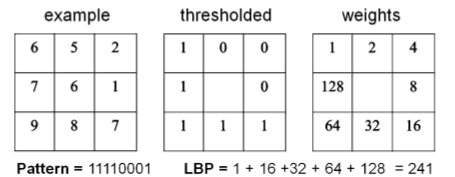
\includegraphics[scale=0.5]{lbp.png}
\caption{LBP 3 x 3 (Pietik\"ainen, Hadid, Zhao \& Ahonen (2011))}
\end{figure}

Notice that the pattern will be come of the form 01001110. This is done when a
the value of the evaluated pixel is greater than the threshold, shift the bit
by the n(with i=i$_{th}$ pixel evaluated, starting with $i=0$).

This results in a mathematical expression:
Let I($x_i, y_i$) an Image with grayscale values and $g_n$ the grayscale value
of the pixel $(x_i, y_i)$. Also let $s(g_i - g_c)$ with $g_c$ = grayscale value
of the center pixel.

$$
  s(v, g_c) = \left\{
  \begin{array}{l l}
    1 & \quad \text{if v $\geq$ $g_c$}\\
    0 & \quad \text{if v $<$ $g_c$}\\
  \end{array} \right.
$$

$$LBP_{n, g_c = (x_c, y_c)} = \sum\limits_{i=0}^{n-1} s(g_i, g_c)^{2i} $$

The outcome of this operations will be a binary pattern.

\item Given this pattern, the next step is to divide the pattern in cells. The
amount of cells depends on the quality of the result, so trial and error is in
order. Starting with dividing the pattern in to cells of size 16. 

\item Compute a histogram for each cell.

\begin{figure}[h!]
\center
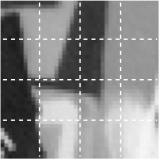
\includegraphics[scale=0.7]{cells.png}
\caption{Divide in cells(Pietik\"ainen et all (2011))}
\end{figure}

\item Consider every histogram as a vector element and concatenate these. The
result is a feature vector of the image.

\item Feed these vectors to a support vector machine. This will ''learn'' which
vector indicate what letter. 

\end{itemize}

To our knowledge, LBP has yet not been used in this manner before. Therefore,
it will be the first thing to implement, to see if it lives up to the
expectations. When the proof of concept is there, it can be used in the final
program.

Important to note is that due to the normalization of characters before
applying LBP. Therefore, no further normalization is needed on the histograms.

Given the LBP of a character, a Support Vector Machine can be used to classify
the character to a character in a learning set. The SVM uses

\subsection{Matching the database}

Given the LBP of a character, a Support Vector Machine can be used to classify
the character to a character in a learning set. The SVM uses the collection of
histograms of an image as a feature vector.  The SVM can be trained with a
subsection of the given dataset called the ''Learning set''. Once trained, the
entire classifier can be saved as a Pickle object\footnote{See
\url{http://docs.python.org/library/pickle.html}} for later usage.

\section{Implementation}

In this section we will describe our implementations in more detail, explaining
choices we made.

\subsection{Licenseplate retrieval}

In order to retrieve the license plate from the entire image, we need to
perform a perspective transformation. However, to do this, we need to know the 
coordinates of the four corners of the licenseplate. For our dataset, this is
stored in XML files. So, the first step is to read these XML files.

\paragraph*{XML reader}

The XML reader will return a 'license plate' object when given an XML file. The
licence plate holds a list of, up to six, NormalizedImage characters and from
which country the plate is from. The reader is currently assuming the XML file
and image name are corresponding. Since this was the case for the given
dataset. This can easily be adjusted if required. 

To parse the XML file, the minidom module is used. So the XML file can be
treated as a tree, where one can search for certain nodes. In each XML
file it is possible that multiple versions exist, so the first thing the reader
will do is retrieve the current and most up-to-date version of the plate. The
reader will only get results from this version.

Now we are only interested in the individual characters so we can skip the
location of the entire license plate. Each character has 
a single character value, indicating what someone thought what the letter or
digit was and four coordinates to create a bounding box. To make things not to
complicated a Character class and Point class are used. They
act pretty much as associative lists, but it gives extra freedom on using the
data. If less then four points have been set the character will not be saved.

When four points have been gathered the data from the actual image is being
requested. For each corner a small margin is added (around 3 pixels) so that no
features will be lost and minimum amounts of new features will be introduced by
noise in the margin. 

In the next section you can read more about the perspective transformation that
is being done. After the transformation the character can be saved: Converted
to grayscale, but nothing further. This was used to create a learning set. If
it doesn't need to be saved as an actual image it will be converted to a
NormalizedImage. When these actions have been completed for each character the
license plate is usable in the rest of the code.

\paragraph*{Perspective transformation}
Once we retrieved the cornerpoints of the license plate, we feed those to a
module that extracts the (warped) license plate from the original image, and
creates a new image where the license plate is cut out, and is transformed to a
rectangle.

\subsection{Noise reduction}

The image contains a lot of noise, both from camera errors due to dark noise 
etc., as from dirt on the license plate. In this case, noise therefore means 
any unwanted difference in color from the surrounding pixels.

\paragraph*{Camera noise and small amounts of dirt}
The dirt on the license plate can be of different sizes. We can reduce the 
smaller amounts of dirt in the same way as we reduce normal noise, by applying
a Gaussian blur to the image. This is the next step in our program.\\
\\
The Gaussian filter we use comes from the \texttt{scipy.ndimage} module. We use
this function instead of our own function, because the standard functions are
most likely more optimized then our own implementation, and speed is an
important factor in this application.

\paragraph*{Larger amounts of dirt}
Larger amounts of dirt are not going to be resolved by using a Gaussian filter.
We rely on one of the characteristics of the Local Binary Pattern, only looking
at the difference between two pixels, to take care of these problems.\\
Because there will probably always be a difference between the characters and
the dirt, and the fact that the characters are very black, the shape of the
characters will still be conserved in the LBP, even if there is dirt
surrounding the character.

\subsection{Character retrieval}

The retrieval of the character is done the same as the retrieval of the license
plate, by using a perspective transformation. The location of the characters on
the license plate is also available in de XML file, so this is parsed from that
as well.

\subsection{Creating Local Binary Patterns and feature vector}



\subsection{Classification}



\section{Finding parameters}

Now that we have a functioning system, we need to tune it to work properly for
license plates. This means we need to find the parameters. Throughout the 
program we have a number of parameters for which no standard choice is
available. These parameters are:\\
\\
\begin{tabular}{l|l}
	Parameter 			& Description\\
	\hline
	$\sigma$  			& The size of the Gaussian blur.\\
	\emph{cell size}	& The size of a cell for which a histogram of LBPs will
	                      be generated.\\
	$\gamma$			& Parameter for the Radial kernel used in the SVM.\\
	$c$					& The soft margin of the SVM. Allows how much training
						  errors are accepted.
\end{tabular}\\
\\
For each of these parameters, we will describe how we searched for a good
value, and what value we decided on.

\subsection{Parameter $\sigma$}

The first parameter to decide on, is the $\sigma$ used in the Gaussian blur. To
find this parameter, we tested a few values, by checking visually what value
removed most noise out of the image, while keeping the edges sharp enough to
work with. By checking in the neighbourhood of the value that performed best,
we where able to 'zoom in' on what we thought was the best value. It turned out
that this was $\sigma = ?$.

\subsection{Parameter \emph{cell size}}

The cell size of the Local Binary Patterns determines over what region a
histogram is made. The trade-off here is that a bigger cell size makes the
classification less affected by relative movement of a character compared to
those in the learning set, since the important structure will be more likely to
remain in the same cell. However, if the cell size is too big, there will not
be enough cells to properly describe the different areas of the character, and
the feature vectors will not have enough elements.\\
\\
In order to find this parameter, we used a trial-and-error technique on a few
basic cell sizes, being ?, 16, ?. We found that the best result was reached by
using ??.

\subsection{Parameters $\gamma$ \& $c$}

The parameters $\gamma$ and $c$ are used for the SVM. $c$ is a standard
parameter for each type of SVM, called the 'soft margin'. This indicates how
exact each element in the learning set should be taken. A large soft margin
means that an element in the learning set that accidentally has a completely
different feature vector than expected, due to noise for example, is not taken
into account. If the soft margin is very small, then almost all vectors will be
taken into account, unless they differ extreme amounts.\\
$\gamma$ is a variable that determines the size of the radial kernel, and as
such blablabla.\\
\\
Since these parameters both influence the SVM, we need to find the best
combination of values. To do this, we perform a so-called grid-search. A
grid-search takes exponentially growing sequences for each parameter, and
checks for each combination of values what the score is. The combination with
the highest score is then used as our parameters, and the entire SVM will be
trained using those parameters.\\
\\
We found that the best values for these parameters are $c=?$ and $\gamma =?$.

\section{Results}

The goal was to find out two things with this research: The speed of the
classification and the accuracy. In this section we will show our findings.

\subsection{Speed}

Recognizing license plates is something that has to be done fast, since there
can be a lot of cars passing a camera in a short time, especially on a highway.
Therefore, we measured how well our program performed in terms of speed. We
measure the time used to classify a license plate, not the training of the
dataset, since that can be done offline, and speed is not a primary necessity
there.\\
\\
The speed of a classification turned out to be blablabla.

\subsection{Accuracy}

Of course, it is vital that the recognition of a license plate is correct,
almost correct is not good enough here. Therefore, we have to get the highest
accuracy score we possibly can.\\
\\ According to Wikipedia
\footnote{
\url{http://en.wikipedia.org/wiki/Automatic_number_plate_recognition}},
commercial license plate recognition software score about $90\%$ to $94\%$,
under optimal conditions and with modern equipment. Our program scores an
average of blablabla.

\section{Difficulties}

During the implementation and testing of the program, we did encounter a
number of difficulties. In this section we will state what these difficulties
were and whether we were able to find a proper solution for them.

\subsection*{Dataset}

We did experience a number of problems with the provided dataset. A number of
these are problems to be expected in a real world problem, but which make
development harder. Others are more elemental problems.\\
The first problem was that the dataset contains a lot of license plates which
are problematic to read, due to excessive amounts of dirt on them. Of course,
this is something you would encounter in the real situation, but it made it
hard for us to see whether there was a coding error or just a bad example.\\
Another problem was that there were license plates of several countries in
the dataset. Each of these countries has it own font, which also makes it
hard to identify these plates, unless there are a lot of these plates in the
learning set.\\
A problem that is more elemental is that some of the characters in the dataset
are not properly classified. This is of course very problematic, both for
training the SVM as for checking the performance. This meant we had to check
each character whether its description was correct.

\subsection*{SVM}

We also had trouble with the SVM for Python. The standard Python SVM, libsvm,
had a poor documentation. There was no explanation what so ever on which
parameter had to be what. This made it a lot harder for us to see what went
wrong in the program.

\section{Workload distribution}

The first two weeks were team based. Basically the LBP algorithm could be
implemented in the first hour, while some talked and someone did the typing.
Some additional 'basics' where created in similar fashion. This ensured that
every team member was up-to-date and could start figuring out which part of the
implementation was most suited to be done by one individually or in a pair.

\subsection{Who did what}
Gijs created the basic classes we could use and helped the rest everyone by 
keeping track of what required to be finished and whom was working on what. 
Tadde\"us and Jayke were mostly working on the SVM and all kinds of tests
whether the histograms were matching and alike. Fabi\"en created the functions
to read and parse the given xml files with information about the license
plates. Upon completion all kinds of learning and data sets could be created.

%Richard je moet even toevoegen wat je hebt gedaan :P:P
%maar miss is dit hele ding wel overbodig. Ik dacht dat Rein het zei tijdens
%gesprek van ik wil weten hoe het ging enzo

\subsection{How it went}

Sometimes one cannot hear the alarm bell and wake up properly. This however was
not a big problem as no one was affraid of staying at Science Park a bit longer
to help out. Further communication usually went through e-mails and replies
were instantaneous! A crew to remember.

\section{Conclusion}

Awesome


\end{document}
